\documentclass[a4paper,12pt]{article}
\usepackage[utf8]{inputenc}
\usepackage{graphicx}
\usepackage{fancyhdr}
\usepackage{amsmath}
\usepackage{adjustbox}
\usepackage{mathtools}
\usepackage{float}
\usepackage[spanish, es-nodecimaldot]{babel} 
\usepackage{lastpage}
\usepackage{amssymb} % Para símbolos matemáticos adicionales
\usepackage{hyperref}
\usepackage{cleveref}
%\usepackage[none]{hyphenat}
\usepackage{array}
\usepackage{listings}
\usepackage{xcolor}

\usepackage{multirow}
\usepackage{textcomp}
\usepackage[left=2.5cm, right=2.5cm, top=3cm, bottom=3cm]{geometry}

\lstset{ 
    language=Matlab,                     % El lenguaje del código
    basicstyle=\ttfamily\footnotesize,                % Tipo de letra
    keywordstyle=\color{blue},           % Color para palabras clave
    commentstyle=\color{green!60!black}, % Color para comentarios
    numbers=left,                        % Numeración de las líneas
    numberstyle=\tiny\color{gray},       % Estilo para los números
    stepnumber=1,                        % Mostrar número en cada línea
    tabsize=4,                           % Tamaño de tabulación
    breaklines=true,                     % Partir líneas largas
    showspaces=false,                    % No mostrar los espacios en blanco
    showstringspaces=false,              % No mostrar espacios dentro de strings
    showtabs=false,                      % No mostrar tabs
}

\graphicspath{{Imagenes/}}

% Encabezado y pie de página
\pagestyle{fancy}
\fancyhf{}
\setlength{\headheight}{30 pt}
\renewcommand{\headrulewidth}{0.2pt}
\fancyhead[R]{\begin{tabular}{@{}l@{}}
\includegraphics[scale=0.4]{escudo.PNG}\end{tabular}}
\fancyhead[L]{\begin{tabular}{@{}c@{}} \textbf{Robótica I - Año: 2024} \\ Trabajo Práctico 8: Planificación y Generación de Trayectorias \end{tabular}}


\fancyfoot[R]{\thepage}
\fancyfoot[C]{\begin{tabular}{@{}c@{}}\textbf{BORQUEZ PEREZ Juan Manuel}\\ \textbf{Legajo 13567}\end{tabular}}
\renewcommand{\footrulewidth}{0.2pt}

\begin{document}

\begin{titlepage}
    \centering
    \vspace*{5cm}
    {\Huge\bfseries Informe de Trabajo Práctico N°8}\\
    \vspace{0.2cm}
    {\Large \textbf{Planificación y Generación de Trayectorias}}\\
    \vspace{0.5cm}
    {\Large Robótica I}\\
    \vspace{0.5 cm}
    {\Large Ingeniería en Mecatrónica}\\
    \vspace{0.2 cm}
    {\Large Facultad de Ingeniería - UNCUYO}\\
    \vspace{1.5cm}
    Alumno: Juan Manuel BORQUEZ PEREZ\\
    Legajo: 13567\\
    \vfill
    {\begin{tabular}{@{}c@{}}
\includegraphics[scale=0.4]{escudo.PNG}\end{tabular}}\hspace{10pt}
    %Año 2023
\end{titlepage}

\section{Ejercicio 1:  Generación de trayectoria entre 2 puntos articulares}
\subsection{Interpolación.}
La interpolación con ``jtraj'' es interpolación quintuple en el espacio articular.
Se indica la posición articular inicial y final y un vector de tiempos (como en este caso) o 
un número de puntos en la discretización (como en el ejercicio siguiente). Cuando se da un vector de tiempos,
la trayectoria se da evaluada en esos instántes y cuando 
se indica un número de puntos, la trayectoria se da evaluada en intervalos equi-espaciados en un tiempo unitario.

\begin{lstlisting}
    % Inciso 1
    q0  = [0     -pi/2     0    0    0 0];  % Posicion inicial
    q1  = [-pi/3 pi/10 -pi/5 pi/2 pi/4 0];  % Posicion final
    ti  = 0;                                % Instante inicial
    tf  = 3;                                % Instante final
    dt  = 0.1;                              % Paso de tiempo
    t   = ti:dt:tf;                         % 3 seg. y una decima de paso
    [Q, QD, QDD]  = jtraj(q0, q1, t);       % Trayectoria interpolada
\end{lstlisting}

La trayectoria interpolada ``Q'' es de 31 X 6 y tiene en filas
la sucesión de posiciones articulares entre la inicial
y la final, incluyéndolas.
Concuerda con el límite y paso de tiempo. Esto es, en 3 segundos
hay 30 decimas y al considerar el instante inicial se tienen 31 puntos.

Las matrices ``QD'' y ``QDD'' son de velocidad y aceleración articular respectivamente 
y tienen las mismas dimensiones que ``Q''.

\subsection{Animación}
Se muestra la trayectoria trazada en \cref{animacion fanuc 1}
\begin{lstlisting}
    % Inciso 2
    figure(1);
    for q = Q'
        fanuc.animate(q');
        pause(dt);
    end
\end{lstlisting}

\subsection{Grafico de las variables articulares.}
\begin{lstlisting}
    %% Inciso 3
    figure(2);
    qplot(t', Q);
\end{lstlisting}

Se puede ver en \cref{qplot fanuc} que el movimiento de los ejes es simultáneo
y síncrono, es decir, que los ejes comienzan su movimiento en el mismo instánte de tiempo
y también lo terminan en el mismo instante de tiempo.

\begin{figure}[H]
    \centering
    \begin{adjustbox}{scale = 0.65, max width=\columnwidth}
        \framebox{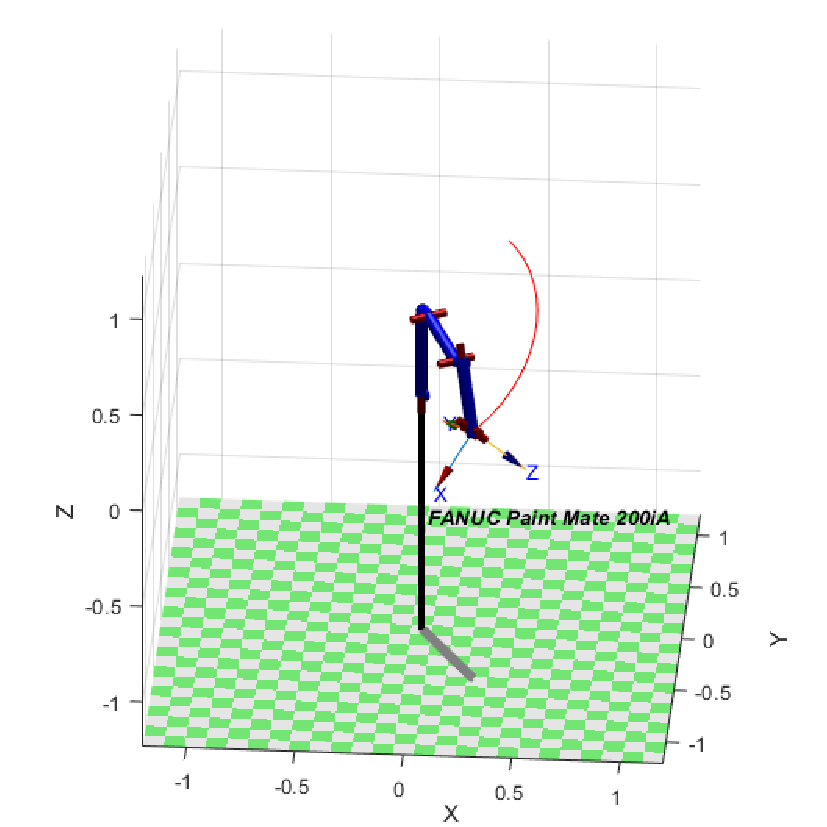
\includegraphics{1-Animacion_Fanuc.pdf}}
    \end{adjustbox}
    \caption{Animación Fanuc.}
    \label{animacion fanuc 1}
\end{figure}

\begin{figure}[H]
    \centering
    \begin{adjustbox}{scale = 0.65, max width=\columnwidth}
        \framebox{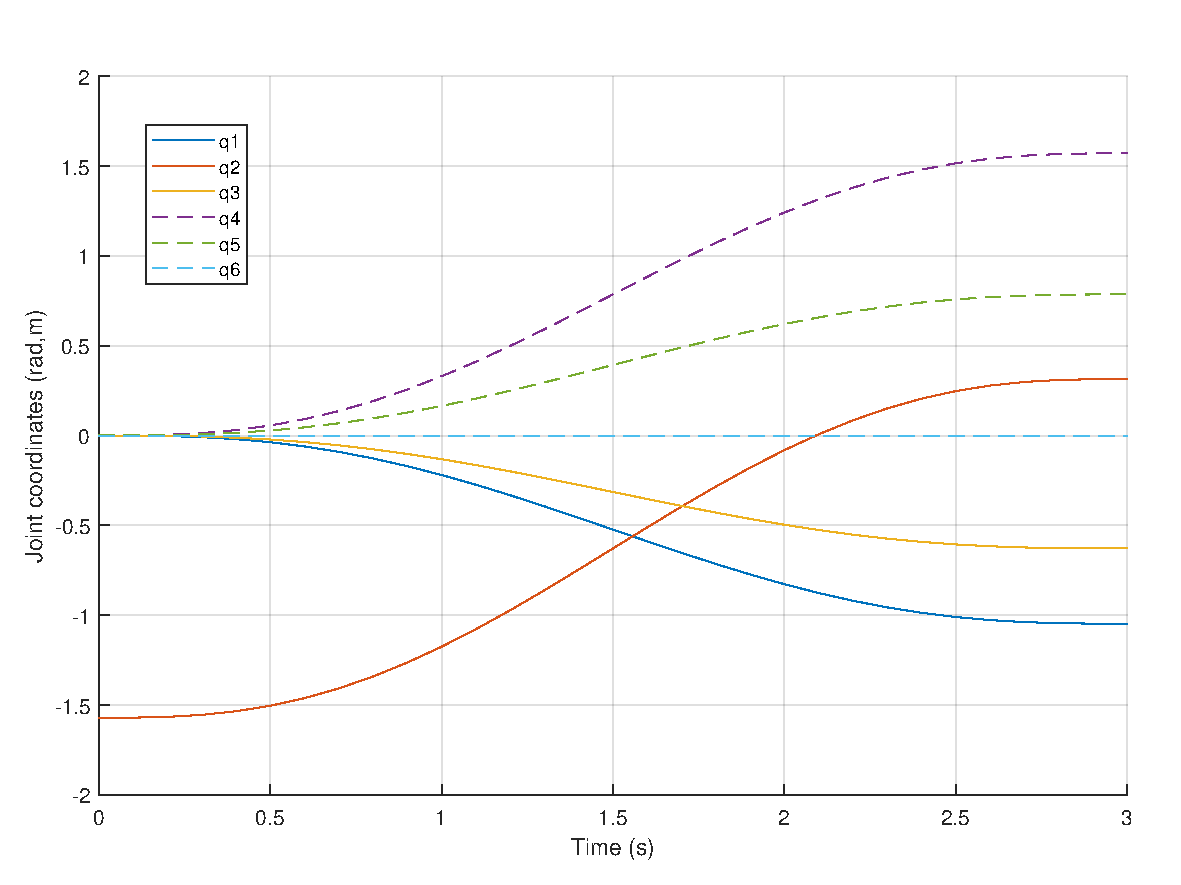
\includegraphics{2-qplot_Fanuc.pdf}}
    \end{adjustbox}
    \caption{qplot Fanuc.}
    \label{qplot fanuc}
\end{figure}

\section{Ejercicio 2: Generación de Trayectorias entre puntos cartesianos. Interpolación articular.}
\subsection{Generación}
\begin{lstlisting}
    %% Inciso 1
    p1 = [0.0 0.0 0.95];            % Posicion incial
    p2 = [0.4 0.0 0.95];            % Posicion final
    qq = [0 -pi/2 -pi/4 0 pi/4 0];  % Posicion articular que da la Orientacion
    R  = fanuc.fkine(qq);           % Matriz homog. que da la Orientacion

    T1 = R; T1.t = p1;              % Postura inicial
    T2 = R; T2.t = p2;              % Postura final

    q1   = fanuc.ikine(T1, 'q0', qq, 'mask', ones(1, 6));
    q2   = fanuc.ikine(T2, 'q0', qq, 'mask', ones(1, 6));

    Q  = jtraj(q1, q2, 100);
\end{lstlisting}

Primero se hace la cinemática directa con ``qq'' . De la matriz ``R'' obtenida,
solo se cambia el vector de traslación por ``p1'' para dar ``T1'' (postura inicial) y por ``p2'' para dar ``T2'' (postura final)
conservando la sub-matriz de rotación.
Luego se usa cinemática inversa para obtener las posiciones articulares correspondientes ``q1'' y ``q2'', con las que se interpola.

\subsection{Animación y qplot}
\begin{lstlisting}
    %% Inciso 2
    figure(1);
    dt = 0.1;
    for q = Q'
        fanuc.animate(q');
        pause(dt);
    end

    figure(2);
    qplot(Q);
\end{lstlisting}

\begin{figure}[H]
    \centering
    \begin{adjustbox}{scale = 0.65, max width=\columnwidth}
        \framebox{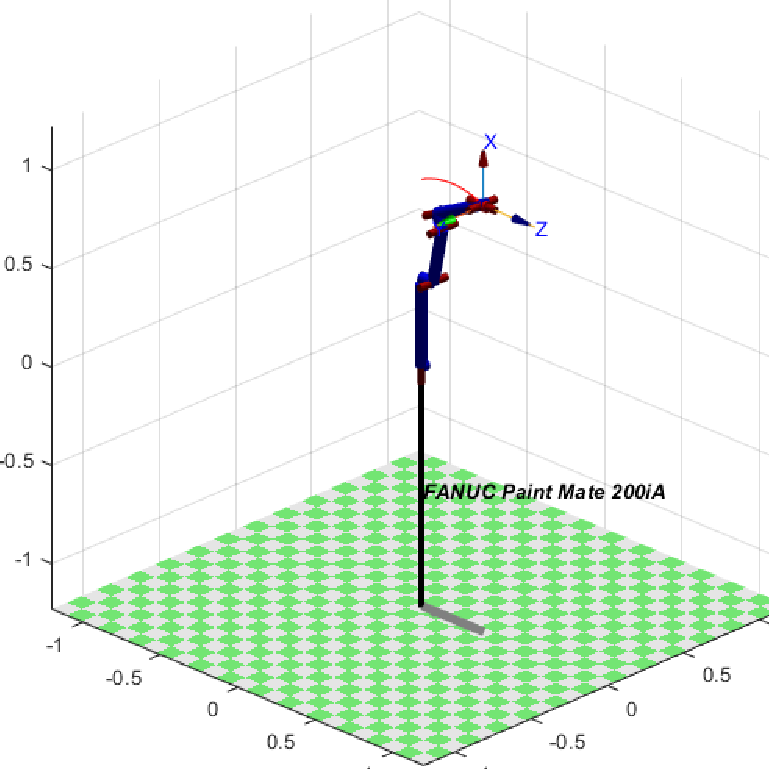
\includegraphics{3-Animacion_Fanuc_2.pdf}}
    \end{adjustbox}
    \caption{Animación Fanuc.}
\end{figure}

\begin{figure}[H]
    \centering
    \begin{adjustbox}{scale = 0.65, max width=\columnwidth}
        \framebox{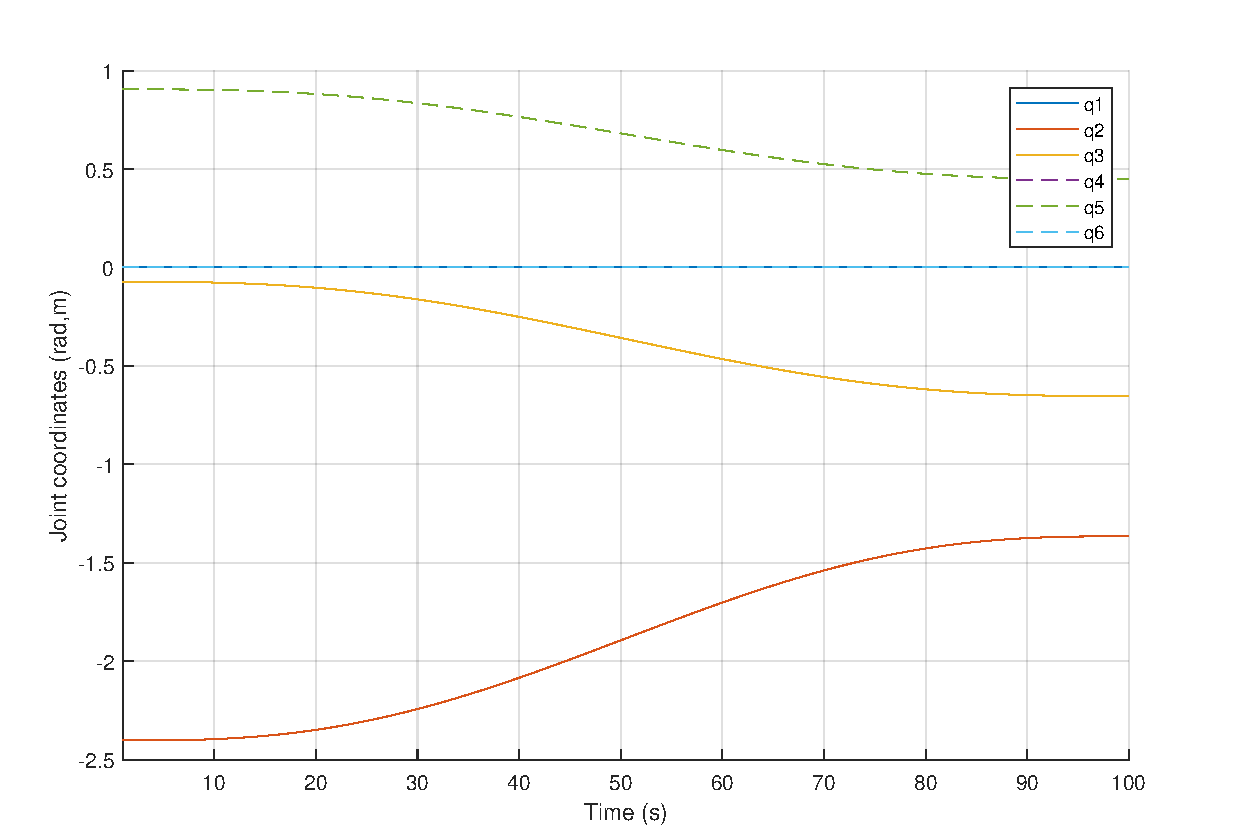
\includegraphics{4-qplot_Fanuc_2.pdf}}
    \end{adjustbox}
    \caption{qplot Fanuc.}
    \label{qplot fanuc}
\end{figure}

\section{Ejercicio 3:  Generación de trayectorias entre 2 puntos cartesianos, interpolación cartesiana}
\subsection{Interpolación con ctraj}
La interpolación con ``ctraj'' es interpolación cartesiana entre dos posturas en una trayectoria recta siguiendo un perfil de velocidad trapezoidal.
Se indican la postura inicial y final con las matrices de transformación homogénea correspondientes y un número de puntos
en la discretización o un vector con fracciones de segmento.
Cuando se indica un vector de fracciones, la interpolación es evaluada 
en esas fracciones a lo largo de la trayectoria.
El resultado de la interpolación es la secuencia de matrices de transformación homogenea.

\begin{lstlisting}
    %% Inciso 1
    p1 = [0.0 0.0 0.95];            % Posicion incial
    p2 = [0.4 0.0 0.95];            % Posicion final
    qq = [0 -pi/2 -pi/4 0 pi/4 0];  % Posicion articular que da la Orientacion
    R  = fanuc.fkine(qq);           % Matriz homog. que da la Orientacion

    T1 = R; T1.t = p1;              % Postura inicial
    T2 = R; T2.t = p2;              % Postura final
    M  = 100;                       % Numero de puntos en la interpolacion

    T  = ctraj(T1, T2, M);          % Trayectoria interpolada

    % Trayectoria en coordenadas articulares
    Q   = fanuc.ikine(T, 'q0', qq, 'mask', ones(1, 6));
\end{lstlisting}

\subsection{Animación y qplot}
\begin{lstlisting}
    %% Inciso 2
    % Trayectoria en coordenadas articulares
    Q   = fanuc.ikine(T, 'q0', qq, 'mask', ones(1, 6));

    figure(1);
    fanuc.plot(Q(1, :), 'scale', 0.65,'jointdiam', 0.65, 'trail', {'r', 'LineWidth', 0.1});
    fprintf("\nPresione ENTER para visualizar la animacion del robot.\n");
    pause;

    dt = 0.1;
    for q = Q'
        fanuc.animate(q');
        pause(dt);
    end

    figure(2);
    qplot(Q);
\end{lstlisting}

\begin{figure}[H]
    \centering
    \begin{adjustbox}{scale = 0.65, max width=\columnwidth}
        \framebox{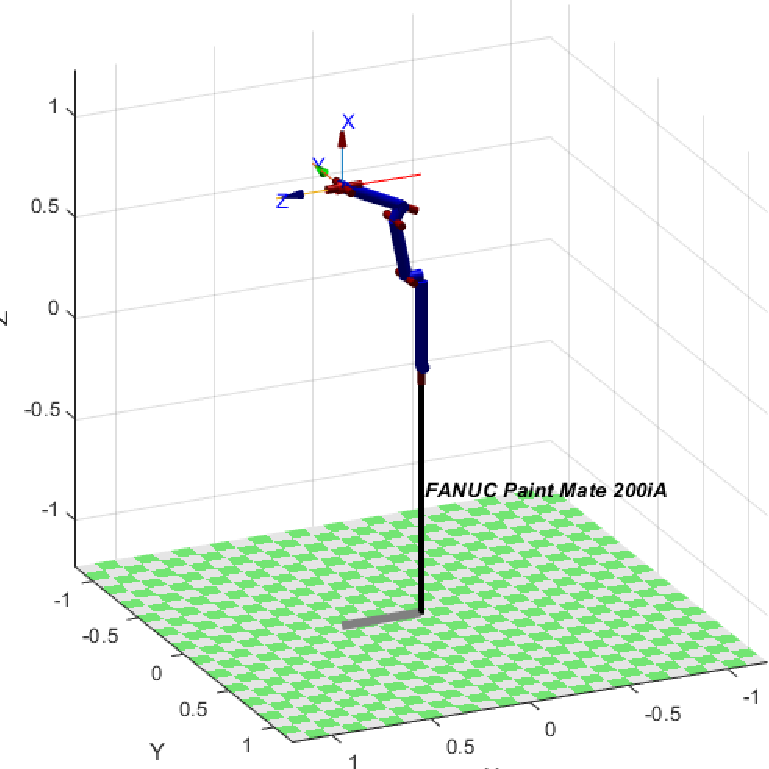
\includegraphics{5-Animacion_Fanuc_3.pdf}}
    \end{adjustbox}
    \caption{Animación Fanuc.}
\end{figure}

\begin{figure}[H]
    \centering
    \begin{adjustbox}{scale = 0.65, max width=\columnwidth}
        \framebox{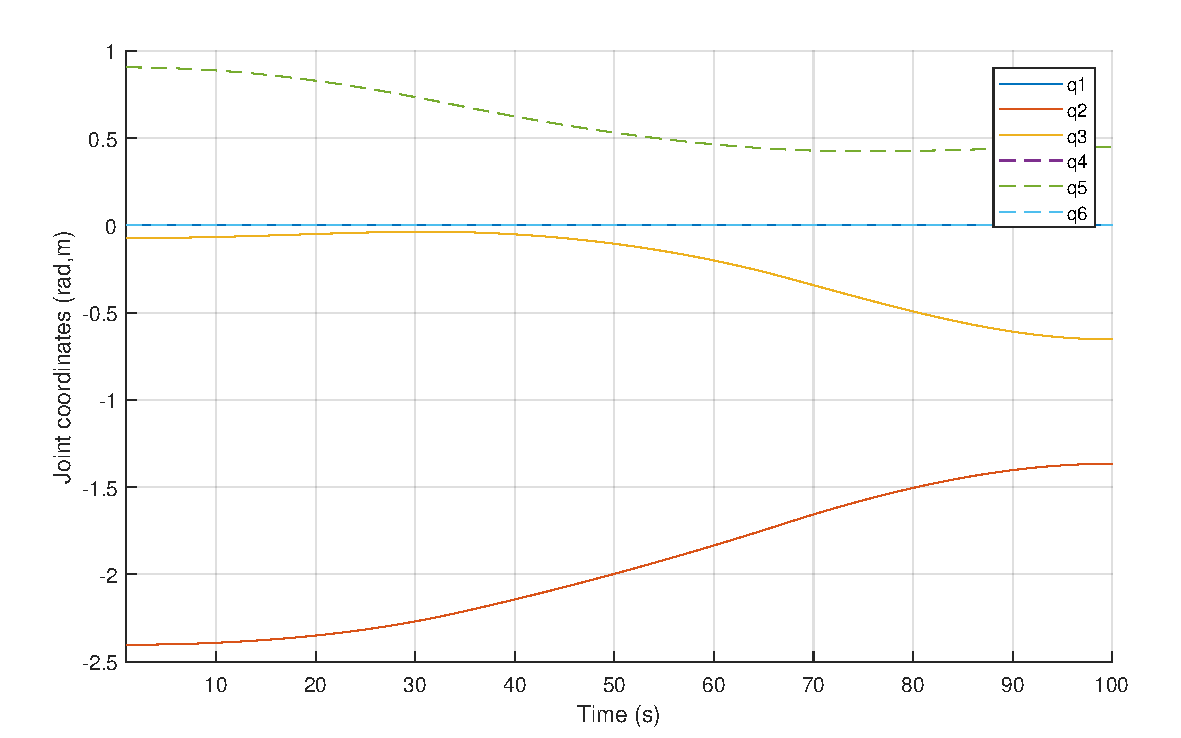
\includegraphics{6-qplot_Fanuc_3.pdf}}
    \end{adjustbox}
    \caption{qplot Fanuc.}
    \label{qplot fanucm 3}
\end{figure}

%\begin{equation*}
%    \prescript{O}{}{Rot_M} = 
%    \begin{bmatrix}
%        0.500 & -0.866\\
%        0.866 & 0.500
%    \end{bmatrix}
%\end{equation*}

%\begin{figure}[H]
%    \centering
%    \begin{adjustbox}{scale = 0.85, max width=\columnwidth}
%        \framebox{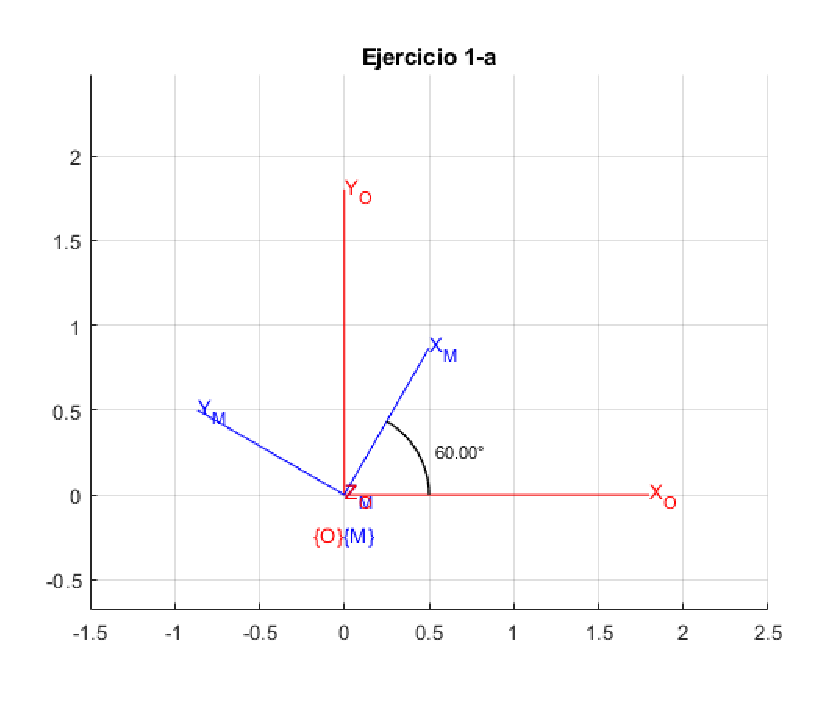
\includegraphics{1-Ejercicio_1_a.pdf}}
%    \end{adjustbox}
%    \caption{Sistema O y Sistema M superpuestos con indicación de ángulo de rotación.}
%\end{figure}


%\begin{table}[H]
%    \centering
%    \begin{tabular}{|c|c|c|c|c|c|}
%    \hline
%    Sistema & $\theta$  & $d$           & $a$    & $\alpha$ & $\sigma$ \\ \hline
%    1       & $q_1$     & $199.2$       & $200$  & 0        & 0        \\ \hline
%    2       & $q_2$     & $59.5$        & $250$  & 0        & 0        \\ \hline
%    3       & $0$       & $q_3$         & $0$    & 180°     & 1        \\ \hline
%    4       & $q_4$     & $37.5$        & $0$    & 0        & 0        \\ \hline
%    \end{tabular}
%    \caption{Parámetros DH alternativos.}
%    \label{parametros DH2}
%\end{table}

\end{document}